% word limit: 500
\section{Results}
\label{sec:results}

\subsection{Velocity dispersion of coeval groups}

To explore the relationship between rotation period, \teff\ and age, we
selected groups of stars within different age ranges \citep[where age was
calculated using the][gyrochronology relation]{angus2019}, and calculated the
velocity dispersion: the standard deviation of velocities in the direction of
increasing galactic latitude, \sigmavb, as a function of effective temperature
for each age group.
We performed 3$\sigma$ sigma-clipping on the stellar velocities in each age
and temperature bin to remove non-Gaussian outliers.
Without sigma-clipping, we found that a small number of high velocity
outliers at the low-temperature end of our sample substantially raised the
velocity dispersion for cooler stars.
Ages were calculated using dereddened \gaia\ \gcolor\ color, however
throughout this paper we show rotation periods as a function of effective
temperature, \teff.
We chose to use \teff and not photometric color in this analysis as it is the
linear quantity and therefore easier to divide into bins of roughly equal
numbers of stars.

\begin{figure}
  \caption{
Top: rotation period vs effective temperature for stars in the \mct\
    catalog.
    The full catalog, with subgiants and visual binaries removed is shown in
    grey, and stars selected to be in different age groups (between \tmin\ and
    \tmax\ K) are overlayed in color.
These age groups were selected using the \citet{angus2019} gyrochronology
    relation.
The legend in the center of the figure lists the age range, in Gyr, of each
    group.
Bottom: velocity dispersion vs effective temperature for each age
    group.
The color of the line corresponds to the color of the group shown in the top
    panel.
If the gyrochronal model were correct at all ages, and the stars in each group
    were the same age across temperatures, the velocity dispersion would be
    constant as a function of \teff.
However, the velocity dispersions of the oldest age groups increase with
    \teff, indicating the \citet{angus2019} gyrochronology model underpredicts
    the the ages of late-K dwarfs relative to the ages of early K dwarfs at
    old ages.
% An alternative explanation could be that the gyrochronology relation is
%     correct and {\it mass-dependent heating} is responsible for the greater
%     velocity dispersions of cooler stars.
}
  \centering
    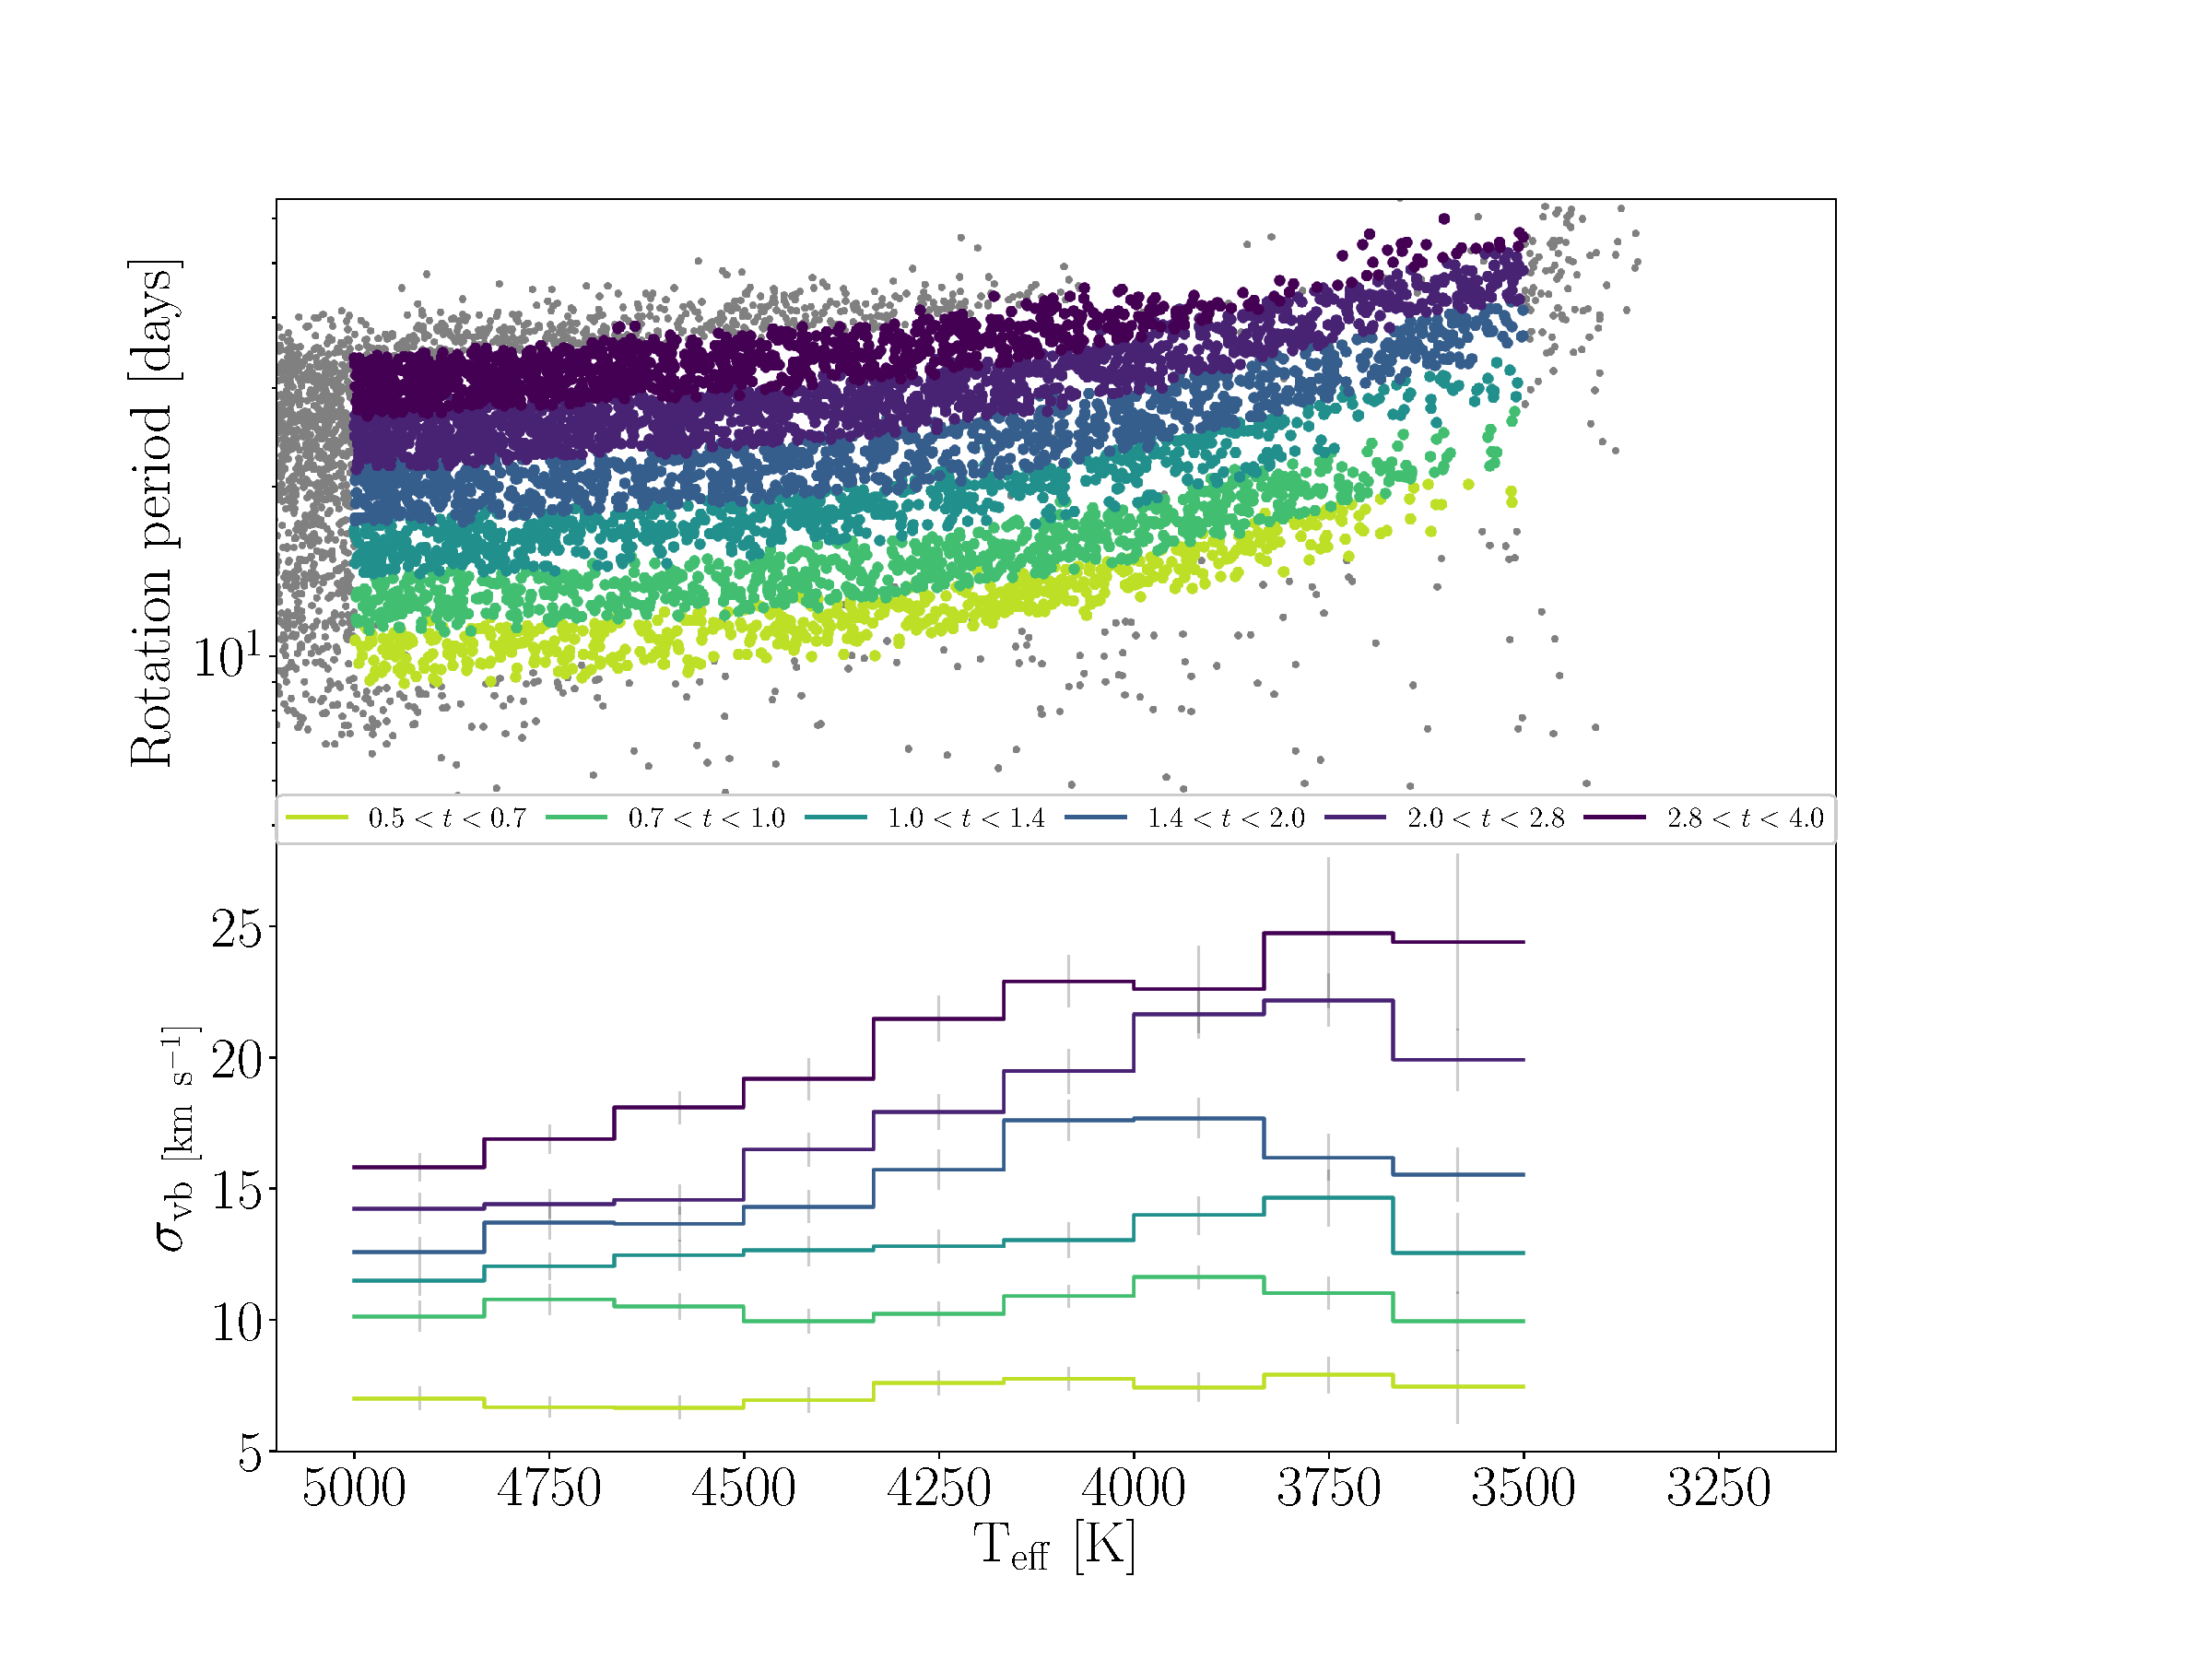
\includegraphics[width=1\textwidth]{age_cut}
\label{fig:age_cut}
\end{figure}
The top panel of figure \ref{fig:age_cut} shows the full \mct\ sample
(excluding visual binaries and subgiants) in grey, with coeval groups shown in
color.
The color of the points corresponds to the age ranges specified in the legend
(in Gyr), which also apply to the lines in the lower panel.
The bottom panel shows the velocity dispersion, \sigmavb\ of each age group,
as a function of effective temperature.
% We only included stars within a temperature range of 5000 - 3500 K in our
% analysis, as hotter stars are more likely to have stopped magnetic braking
% \citep{vansaders2016}, which could bias the results.
Late M dwarfs were not included in our analysis because such faint stars
cannot be observed at large heights above the plane (because of the low
galactic latitude of the \kepler\ field, stars at high-Z are more distant),
which introduces a mass-dependent velocity bias: cooler populations of stars
are skewed towards lower velocity dispersions.
The coolest temperature bins in the lower panel of figure \ref{fig:age_cut}
have low velocity dispersions, indicating that this effect may already become
important at temperatures lower than $\sim$ 4000 K.

Overall, figure \ref{fig:age_cut} shows that velocity dispersion increases
with gyrochronal age across all temperatures, implying that both velocity
dispersion and rotation periods increase with age as expected.
The constant velocity dispersion of young stars as a function of temperature
shows that the Praesepe-calibrated gyrochronology relation accurately predicts
the relative ages of {\it young} field stars.
% To our knowledge, no gyrochronology relation has never been demonstrated to
% correctly predict ages (either relative or absolute) for such cool or such
% young field stars.
% This is not particularly remarkable however, since these young stars are a
% similar age to the Praesepe cluster, which was used to calibrate the
% period-color relation.
% However, if the stars in each selected age group had the {\it same} age across
% the temperature range, their velocity dispersion would be a constant function
% of \teff.
In contrast however, velocity dispersion increases as a function of
temperature for old stars, meaning the \citet{angus2019} gyrochronology
relation underpredicts the ages of old, late-K dwarfs (or overpredicts the
ages of old early-K dwarfs).
This indicates that the relationship between period and photometric
color or \teff\ flattens out over time.
In other words, the lines of constant age sweeping diagonally upwards in the
top panel of figure \ref{fig:age_cut} are too steeply sloped at old ages.

\subsection{The period-\teff\ relations, revealed}

\begin{figure}
  \caption{
      Top: Rotation period vs effective temperature for stars in the \mct\
    sample, colored by the velocity dispersions of stars over a grid in
    $\log_{10}$(period) and \teff.
    Bottom: the velocity dispersions of groups of stars, shown as a solid
    grid for clarity.
    The black solid lines on both panels show a 1.1 Gyr isochrone, calculated
    with the \citet{angus2019} gyrochronology relation which roughly traces
    the rotation period gap.
    The black dashed lines show a 650 Myr isochrone, indicating the location
    and shape of the Praesepe cluster (to which this gyrochronology model was
    calibrated).
    The black points show the 1.1 Gyr NGC 6811 open cluster.
}
  \centering
    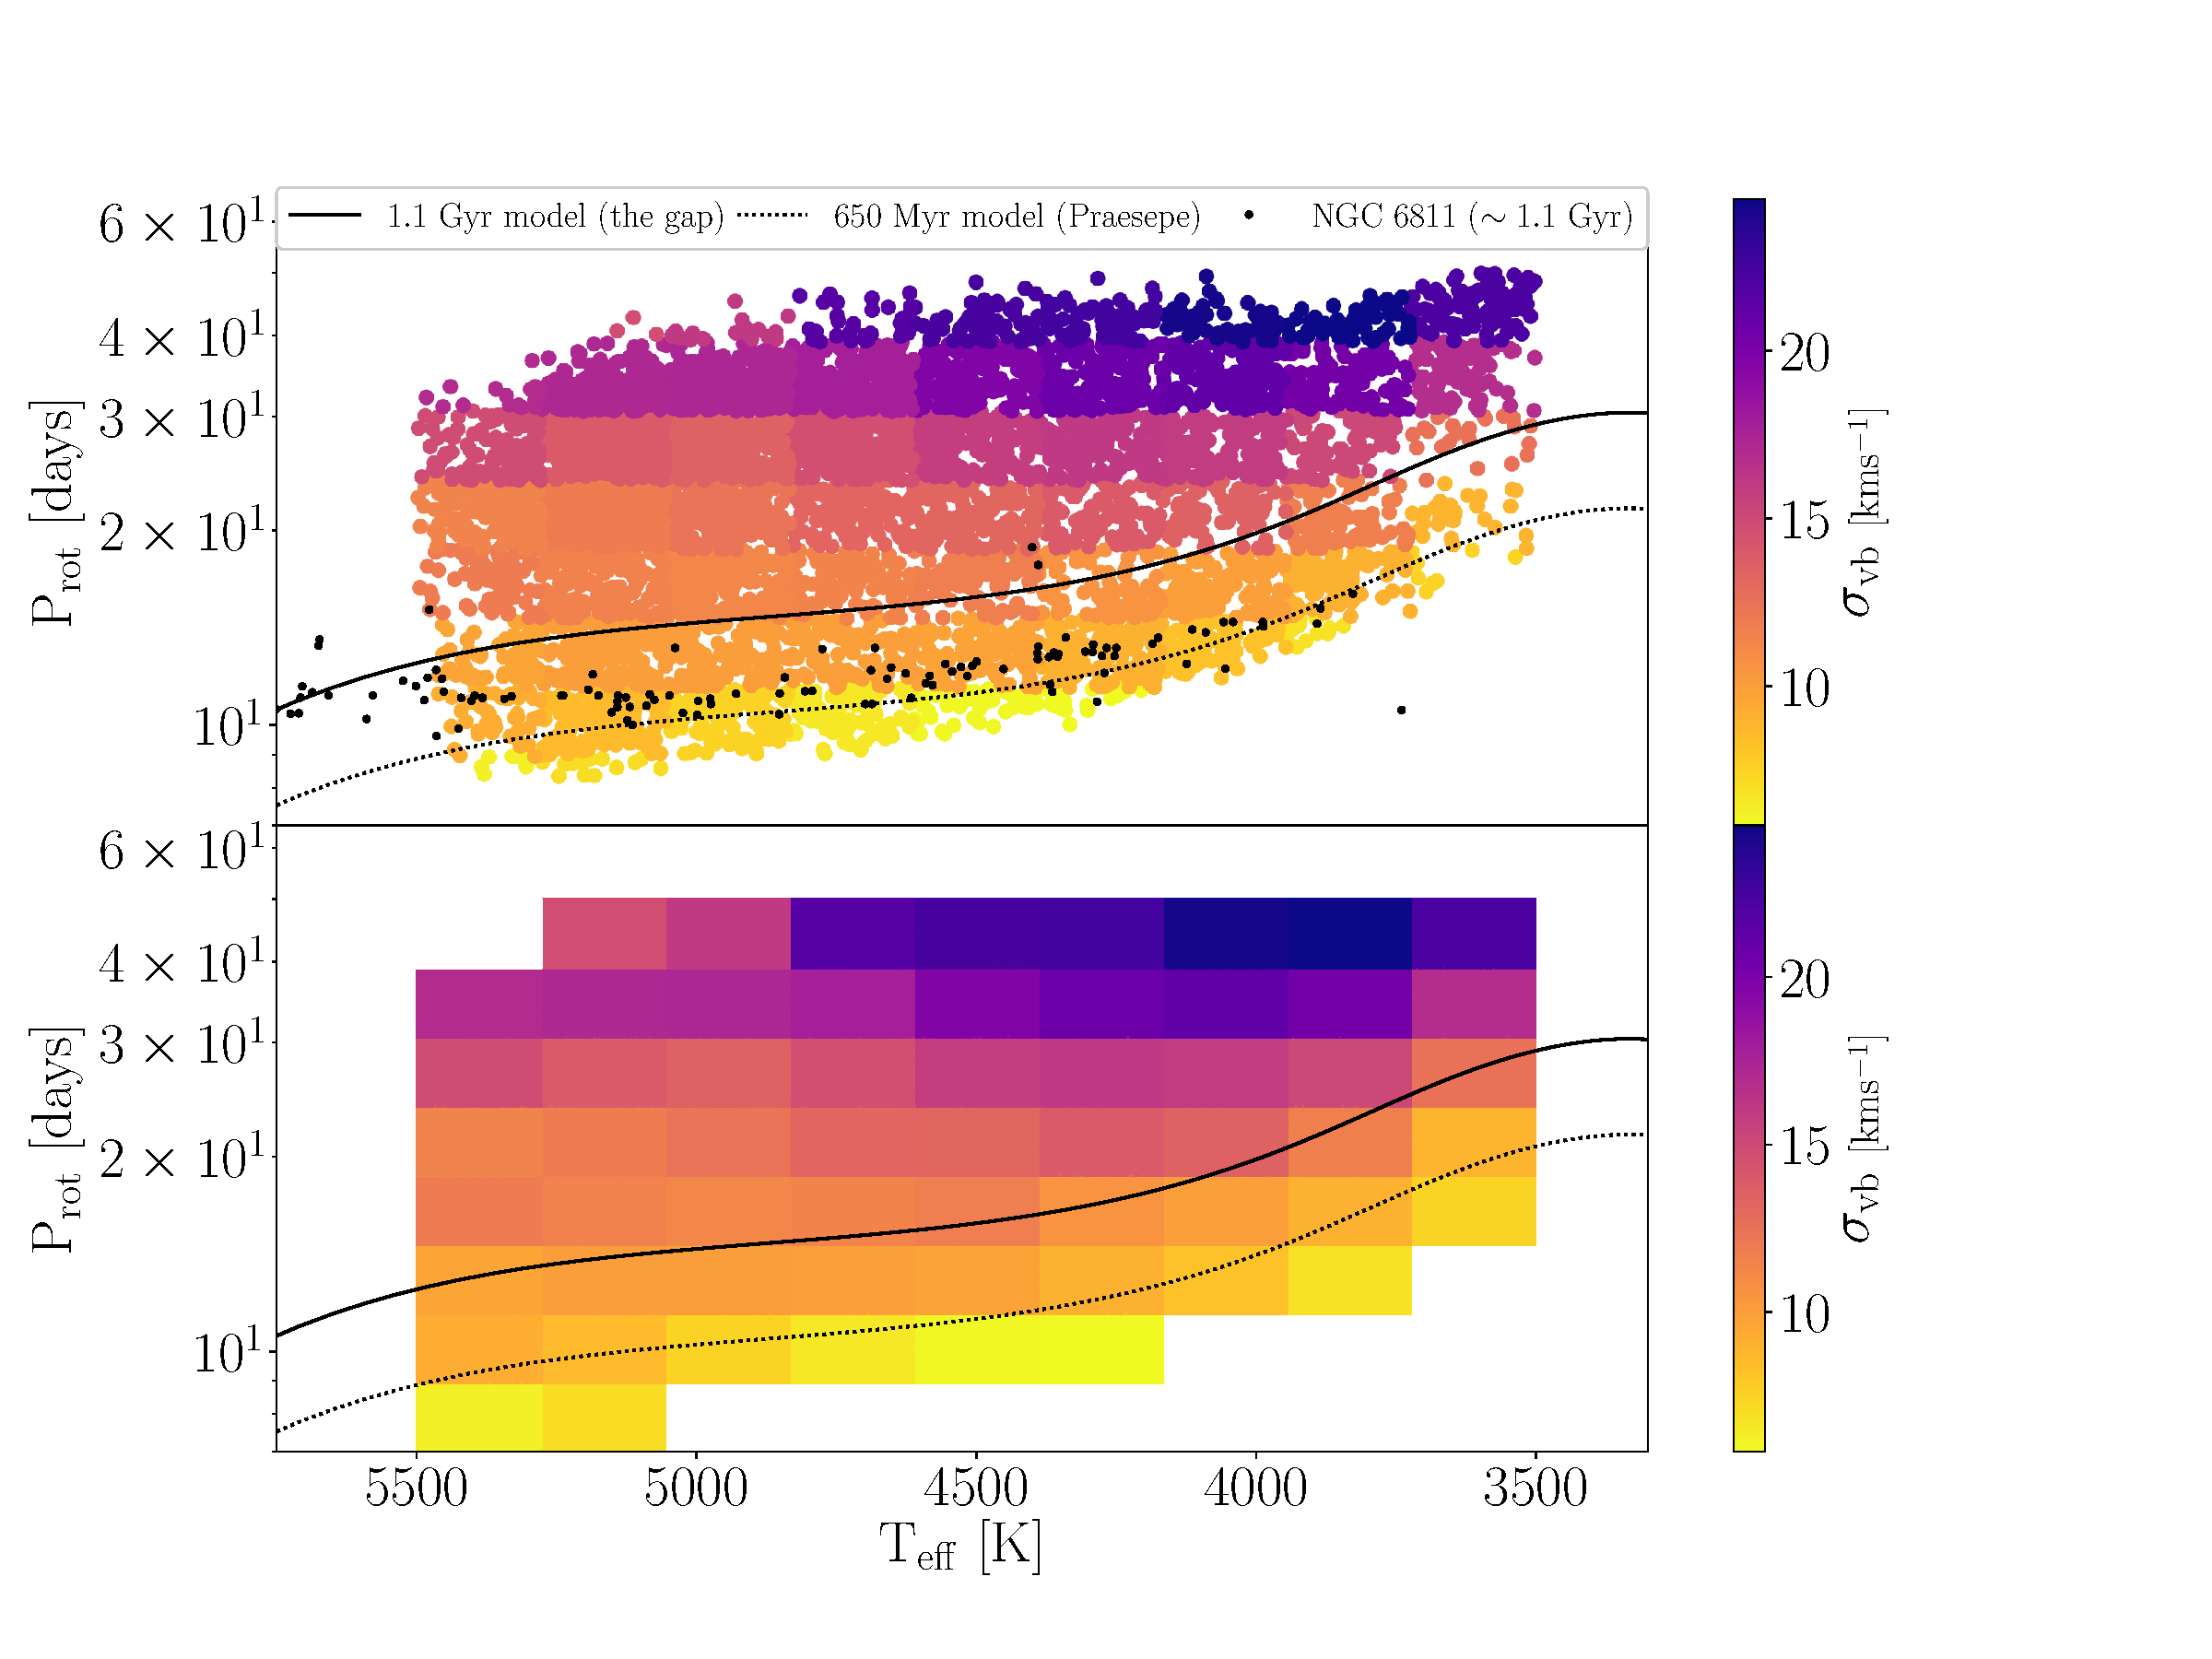
\includegraphics[width=1\textwidth]{vplot}
\label{fig:dispersion_period_teff}
\end{figure}
Figure \ref{fig:dispersion_period_teff} shows rotation period vs. \teff\ for
our sample, coloured by (\vb) velocity dispersion.
Velocity dispersion was calculated for groups of stars over a grid in
$\log_{10}$(period) and temperature.
If we assume that mass dependent heating doesn't affect this sample, and \vb\
at low galactic latitudes is an unbiased tracer of \vz, \vb\ velocity
dispersion can be interpreted as an age proxy and stars plotted in a similar
color in figure \ref{fig:dispersion_period_teff} are similar ages.
Interpreted this way, lines of constant age (isochrones) appear to follow the
shape of the Praesepe-based gyrochronology model (black dotted line) at young
ages.
However, this does not seem to be true age old ages where it appears that
rotation period {\it decreases} with decreasing effective temperatures.
This is a paradigm shift for gyrochronology because stellar spin-down rate is
thought to be directly tied to magnetic field strength, and the deeper
convection zones of cooler stars generate stronger magnetic fields which {\it
should} lead to more efficient angular momentum loss.
% The shape of the upper envelope of rotation periods in the top panels of
% figures \ref{fig:age_cut} and \ref{fig:dispersion_period_teff} also hints at
% this.
The shape of the period-\teff\ relations at old ages appears to follow the
shape of the upper detection edge, with the so-called `M dwarf dip'
\citep{vansaders2018} reflected in the lines of constant velocity dispersion
(and presumed age) in the top panel of figure
\ref{fig:dispersion_period_teff}.
If the shape of that upper edge is created by a detection limit, our results
suggest that stars cooler than $\sim$4500 K become inactive (and their
rotation periods therefore become undetectable) at around the same age, but at
an older age than stars hotter than $\sim$4500.
The (kinematically) oldest stars in the \mct\ sample are cooler than 4500 K.
This is probably because cooler stars remain active for longer, and their
rotation periods can therefore be measured at older ages.

We reiterate that the velocity dispersions of the coolest stars may be
affected by a selection bias -- these extremely faint stars are more difficult
to detect at larger distances, larger heights above the plane, and therefore
larger velocities.
It is possible that some high velocity stars of temperatures cooler than
$\sim$4000 K are missing from this sample, and the velocity dispersions may
therefore appear lower than they truly are.
This could be why the velocity dispersion appears to decrease towards the
right of figure \ref{fig:dispersion_period_teff}.
